\documentclass{article}

% Recommended, but optional, packages for figures and better typesetting:
\usepackage{microtype}
\usepackage{graphicx}
\usepackage{subfigure}
\usepackage{booktabs} % for professional tables

% hyperref makes hyperlinks in the resulting PDF.
% If your build breaks (sometimes temporarily if a hyperlink spans a page)
% please comment out the following usepackage line and replace
% \usepackage{icml2018} with \usepackage[nohyperref]{icml2018} above.
\usepackage{hyperref}

% Attempt to make hyperref and algorithmic work together better:
\newcommand{\theHalgorithm}{\arabic{algorithm}}

% Use the following line for the initial blind version submitted for review:
\usepackage{icml2018}

% If accepted, instead use the following line for the camera-ready submission:
%\usepackage[accepted]{icml2018}

% Custom packages
\usepackage{mathtools}
\usepackage{amssymb}

% The \icmltitle you define below is probably too long as a header.
% Therefore, a short form for the running title is supplied here:
\icmltitlerunning{Wake-Sleep for Probabilistic Programming}

\begin{document}

\twocolumn[
\icmltitle{Wake-Sleep for Probabilistic Programming}

% It is OKAY to include author information, even for blind
% submissions: the style file will automatically remove it for you
% unless you've provided the [accepted] option to the icml2018
% package.

% List of affiliations: The first argument should be a (short)
% identifier you will use later to specify author affiliations
% Academic affiliations should list Department, University, City, Region, Country
% Industry affiliations should list Company, City, Region, Country

% You can specify symbols, otherwise they are numbered in order.
% Ideally, you should not use this facility. Affiliations will be numbered
% in order of appearance and this is the preferred way.
\icmlsetsymbol{equal}{*}

\begin{icmlauthorlist}
\icmlauthor{Aeiau Zzzz}{equal,to}
\icmlauthor{Bauiu C.~Yyyy}{equal,to,goo}
\icmlauthor{Cieua Vvvvv}{goo}
\icmlauthor{Iaesut Saoeu}{ed}
\icmlauthor{Fiuea Rrrr}{to}
\icmlauthor{Tateu H.~Yasehe}{ed,to,goo}
\icmlauthor{Aaoeu Iasoh}{goo}
\icmlauthor{Buiui Eueu}{ed}
\icmlauthor{Aeuia Zzzz}{ed}
\icmlauthor{Bieea C.~Yyyy}{to,goo}
\icmlauthor{Teoau Xxxx}{ed}
\icmlauthor{Eee Pppp}{ed}
\end{icmlauthorlist}

\icmlaffiliation{to}{Department of Computation, University of Torontoland, Torontoland, Canada}
\icmlaffiliation{goo}{Googol ShallowMind, New London, Michigan, USA}
\icmlaffiliation{ed}{School of Computation, University of Edenborrow, Edenborrow, United Kingdom}

\icmlcorrespondingauthor{Cieua Vvvvv}{c.vvvvv@googol.com}
\icmlcorrespondingauthor{Eee Pppp}{ep@eden.co.uk}

% You may provide any keywords that you
% find helpful for describing your paper; these are used to populate
% the "keywords" metadata in the PDF but will not be shown in the document
\icmlkeywords{Machine Learning, ICML}

\vskip 0.3in
]

% this must go after the closing bracket ] following \twocolumn[ ...

% This command actually creates the footnote in the first column
% listing the affiliations and the copyright notice.
% The command takes one argument, which is text to display at the start of the footnote.
% The \icmlEqualContribution command is standard text for equal contribution.
% Remove it (just {}) if you do not need this facility.

%\printAffiliationsAndNotice{}  % leave blank if no need to mention equal contribution
% \printAffiliationsAndNotice{\icmlEqualContribution} % otherwise use the standard text.

\begin{abstract}
\end{abstract}

\section{Introduction}

\section{Background}

\subsection{Inference Compilation}
\subsection{Variational Autoencoders}
\subsection{Wake-Sleep}

\section{Wake-Sleep for Probabilistic Programming}

\subsection{Algorithm}
\subsection{Architecture}
\subsection{No Need for Reparameterization}

\section{Experiments}
\subsection{Gaussian Mixture}
\begin{figure*}[!htb]
    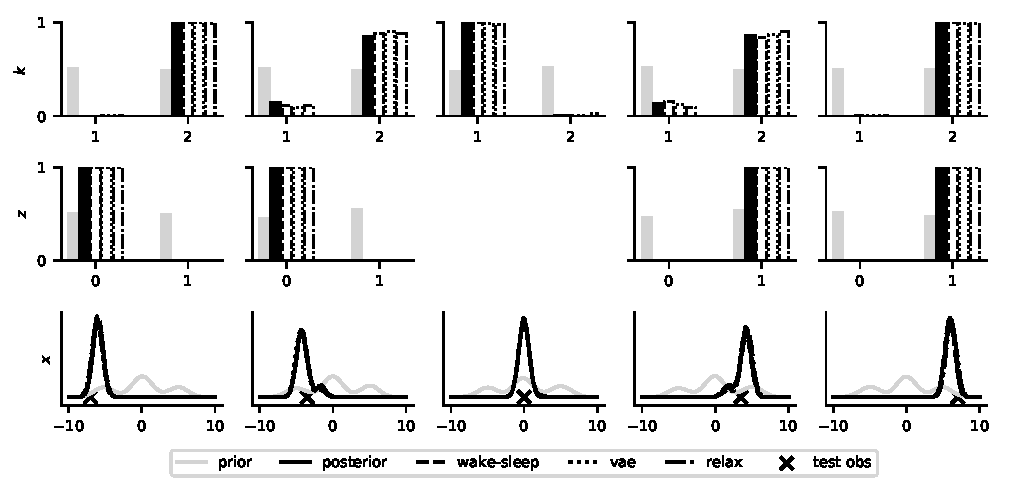
\includegraphics{figures/gmm-open-universe/gmm_open_universe_inference.pdf}
\end{figure*}

\begin{figure}[!htb]
    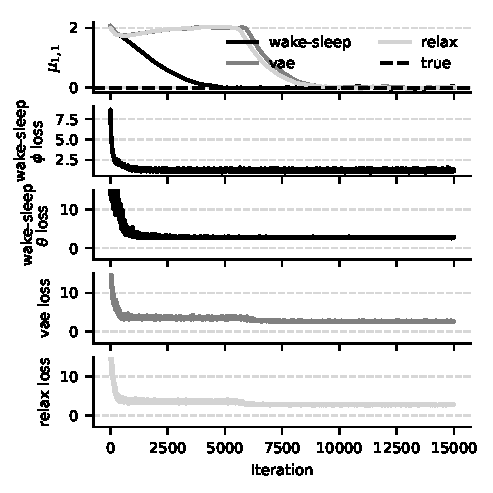
\includegraphics{figures/gmm-open-universe/gmm_open_universe_model_param_and_loss.pdf}
\end{figure}

\subsection{Fly-vs-Fly Dataset}
The Fly-vs-Fly dataset~\citep{eyjolfsdottir2014detecting} contains annotated tracks of pairs of fruit flies interacting.

Given a time series $y_{1:T}$ where $y_t \in \mathbb R^{d_y}$ and $y_t^{\text{pos}} = (y_{t, 1}, y_{t, 2})$, we posit a generative model with $F$ flies and $A$ actions as follows.
\begin{itemize}
    \item For $f$ in $\{1, \dotsc, F\}$:
    \begin{align}
        a_{1, f} &\sim \mathrm{Uniform}(\{1, \dotsc, A\}) \\
        x_{1, f} &\sim \mathrm{Normal}(\mu_{x_1}, \Sigma_{x_1}) \\
        s_{1, f} &\sim \mathrm{Normal}(\mu_{s_1}, \Sigma_{s_1}) \\
        y_{1, f}^{\text{pos}} &\sim \mathrm{Normal}(x_{1, f}, \Sigma_{\text{pos}}) \\
        \mathrm{Enc}(f, y_{1, 1:F}) &\sim \prod_{k = 1}^K \mathrm{Bernoulli}(\eta_k(s_{1, f}))
    \end{align}
    \item For $t$ in $\{2, \dotsc, T\}$:
    \begin{itemize}
        \item For $f$ in $\{1, \dotsc, F\}$:
        \begin{align}
            a_{t, f} &\sim \mathrm{Categorical}(\pi_{a_{t - 1, f}}^a(s_{t, f})) \\
            x_{t, f} &\sim \mathrm{Normal}(\pi_{a_{t - 1, f}}^x(s_{t, f}), \Sigma_x) \\
            s_{t, f} &\sim \mathrm{Normal}(\pi_{a_{t - 1, f}}^s(s_{t, f}, x_{t, f}), \Sigma_s) \\
            y_{t, f}^{\text{pos}} &\sim \mathrm{Normal}(x_{t, f}, \Sigma_{\text{pos}}) \\
            \mathrm{Enc}(f, y_{t, 1:F}) &\sim \prod_{k = 1}^K \mathrm{Bernoulli}(\eta_k(s_{t, f}))
        \end{align}
    \end{itemize}
\end{itemize}
where $a_{t, f}$ represents action of fly $f$ at time $t$, $x_{t, f}$ represents its position, and $s_{1, f}$ represents its mental state.
We fix the hyperparameters $\mu_{x_1}, \Sigma_{x_1}, \mu_{s_1}, \Sigma_{s_1}, \Sigma_{\text{pos}}, \Sigma_x$ and $\Sigma_s$.
The likelihood model consists of a likelihood on the position and a likelihood on the encoding of the field of view of each fly.
The parts of the probabilistic model to be learned are the likelihood neural network $\eta_k$ $(k = 1, \dotsc, k)$ and the policy neural networks $\pi_\alpha^a, \pi_\alpha^x, \pi_\alpha^s$ $(\alpha = 1, \dotsc, A)$.

\paragraph{Encoding of the field of view.}
For each fly $f$ at position $t$, we calculate the encoding of its field of view as follows.
Let $r_k$ be a ray starting at the $y_{t, f}$ extending in the direction $(y_{t, f}^{\text{angle}} -\rho / 2 + \rho / k)$ where $y_{t, f}^{\text{angle}}$ is the angle of orientation of the fly and $\rho$ is the field of view angle.
The $k$th element of $\mathrm{Enc}(f, y_{t, 1:F}) \in \{0, 1\}^K$ is $1$ if there is another fly in the area between $r_{k - 1}$ and $r_k$, and $0$ otherwise.

\section{Discussion}


\bibliography{main}
\bibliographystyle{icml2018}

\end{document}


% This document was modified from the file originally made available by
% Pat Langley and Andrea Danyluk for ICML-2K. This version was created
% by Iain Murray in 2018. It was modified from a version from Dan Roy in
% 2017, which was based on a version from Lise Getoor and Tobias
% Scheffer, which was slightly modified from the 2010 version by
% Thorsten Joachims & Johannes Fuernkranz, slightly modified from the
% 2009 version by Kiri Wagstaff and Sam Roweis's 2008 version, which is
% slightly modified from Prasad Tadepalli's 2007 version which is a
% lightly changed version of the previous year's version by Andrew
% Moore, which was in turn edited from those of Kristian Kersting and
% Codrina Lauth. Alex Smola contributed to the algorithmic style files.
